\documentclass[]{article}
\usepackage{lmodern}
\usepackage{amssymb,amsmath}
\usepackage{ifxetex,ifluatex}
\usepackage{fixltx2e} % provides \textsubscript
\ifnum 0\ifxetex 1\fi\ifluatex 1\fi=0 % if pdftex
  \usepackage[T1]{fontenc}
  \usepackage[utf8]{inputenc}
\else % if luatex or xelatex
  \ifxetex
    \usepackage{mathspec}
  \else
    \usepackage{fontspec}
  \fi
  \defaultfontfeatures{Ligatures=TeX,Scale=MatchLowercase}
\fi
% use upquote if available, for straight quotes in verbatim environments
\IfFileExists{upquote.sty}{\usepackage{upquote}}{}
% use microtype if available
\IfFileExists{microtype.sty}{%
\usepackage{microtype}
\UseMicrotypeSet[protrusion]{basicmath} % disable protrusion for tt fonts
}{}
\usepackage[margin=1in]{geometry}
\usepackage{hyperref}
\hypersetup{unicode=true,
            pdftitle={Appendix B: Supplemental Results},
            pdfauthor={Tim M. Szewczyk, Marek Petrik, Jenica M. Allen},
            pdfborder={0 0 0},
            breaklinks=true}
\urlstyle{same}  % don't use monospace font for urls
\usepackage{graphicx,grffile}
\makeatletter
\def\maxwidth{\ifdim\Gin@nat@width>\linewidth\linewidth\else\Gin@nat@width\fi}
\def\maxheight{\ifdim\Gin@nat@height>\textheight\textheight\else\Gin@nat@height\fi}
\makeatother
% Scale images if necessary, so that they will not overflow the page
% margins by default, and it is still possible to overwrite the defaults
% using explicit options in \includegraphics[width, height, ...]{}
\setkeys{Gin}{width=\maxwidth,height=\maxheight,keepaspectratio}
\IfFileExists{parskip.sty}{%
\usepackage{parskip}
}{% else
\setlength{\parindent}{0pt}
\setlength{\parskip}{6pt plus 2pt minus 1pt}
}
\setlength{\emergencystretch}{3em}  % prevent overfull lines
\providecommand{\tightlist}{%
  \setlength{\itemsep}{0pt}\setlength{\parskip}{0pt}}
\setcounter{secnumdepth}{5}
% Redefines (sub)paragraphs to behave more like sections
\ifx\paragraph\undefined\else
\let\oldparagraph\paragraph
\renewcommand{\paragraph}[1]{\oldparagraph{#1}\mbox{}}
\fi
\ifx\subparagraph\undefined\else
\let\oldsubparagraph\subparagraph
\renewcommand{\subparagraph}[1]{\oldsubparagraph{#1}\mbox{}}
\fi

%%% Use protect on footnotes to avoid problems with footnotes in titles
\let\rmarkdownfootnote\footnote%
\def\footnote{\protect\rmarkdownfootnote}

%%% Change title format to be more compact
\usepackage{titling}

% Create subtitle command for use in maketitle
\providecommand{\subtitle}[1]{
  \posttitle{
    \begin{center}\large#1\end{center}
    }
}

\setlength{\droptitle}{-2em}

  \title{Appendix B: Supplemental Results}
    \pretitle{\vspace{\droptitle}\centering\huge}
  \posttitle{\par}
  \subtitle{The performance of presence-based and process-based species distribution
models under realistic conditions}
  \author{Tim M. Szewczyk, Marek Petrik, Jenica M. Allen}
    \preauthor{\centering\large\emph}
  \postauthor{\par}
    \date{}
    \predate{}\postdate{}
  
\newcommand{\beginsupplement}{\setcounter{table}{0}  \renewcommand{\thetable}{B.\arabic{table}} \setcounter{figure}{0} \renewcommand{\thefigure}{B.\arabic{figure}}}  \usepackage{longtable}  \usepackage{caption}

\begin{document}
\maketitle

{
\setcounter{tocdepth}{1}
\tableofcontents
}
\setcounter{table}{0}  \renewcommand{\thetable}{B.\arabic{table}} \setcounter{figure}{0} \renewcommand{\thefigure}{B.\arabic{figure}}

\begin{center}\rule{0.5\linewidth}{\linethickness}\end{center}

This appendix contains supplemental figures to provide additional detail
for the results, including figures for sensitivity and specificity, and
additional detail on predicted slopes for the IPM and
CA\textsubscript{i} models.

\begin{center}\rule{0.5\linewidth}{\linethickness}\end{center}

\newpage
\section{Sensitivity and specificity}

\subsection{Overall averages}

The True Skill Statistic (TSS) evaluates the combined ability of a model
to predict the presences and the absences. While TSS is useful for
comparing overall performance, the individual components can provide
insight as well. Here, we show summary plots for the effect of each
scenario on the sensitivity (the proportion of true presences correctly
predicted as presences) and specificity (the proportion of true absences
correctly predicted as absences).

\begin{figure}
    \centering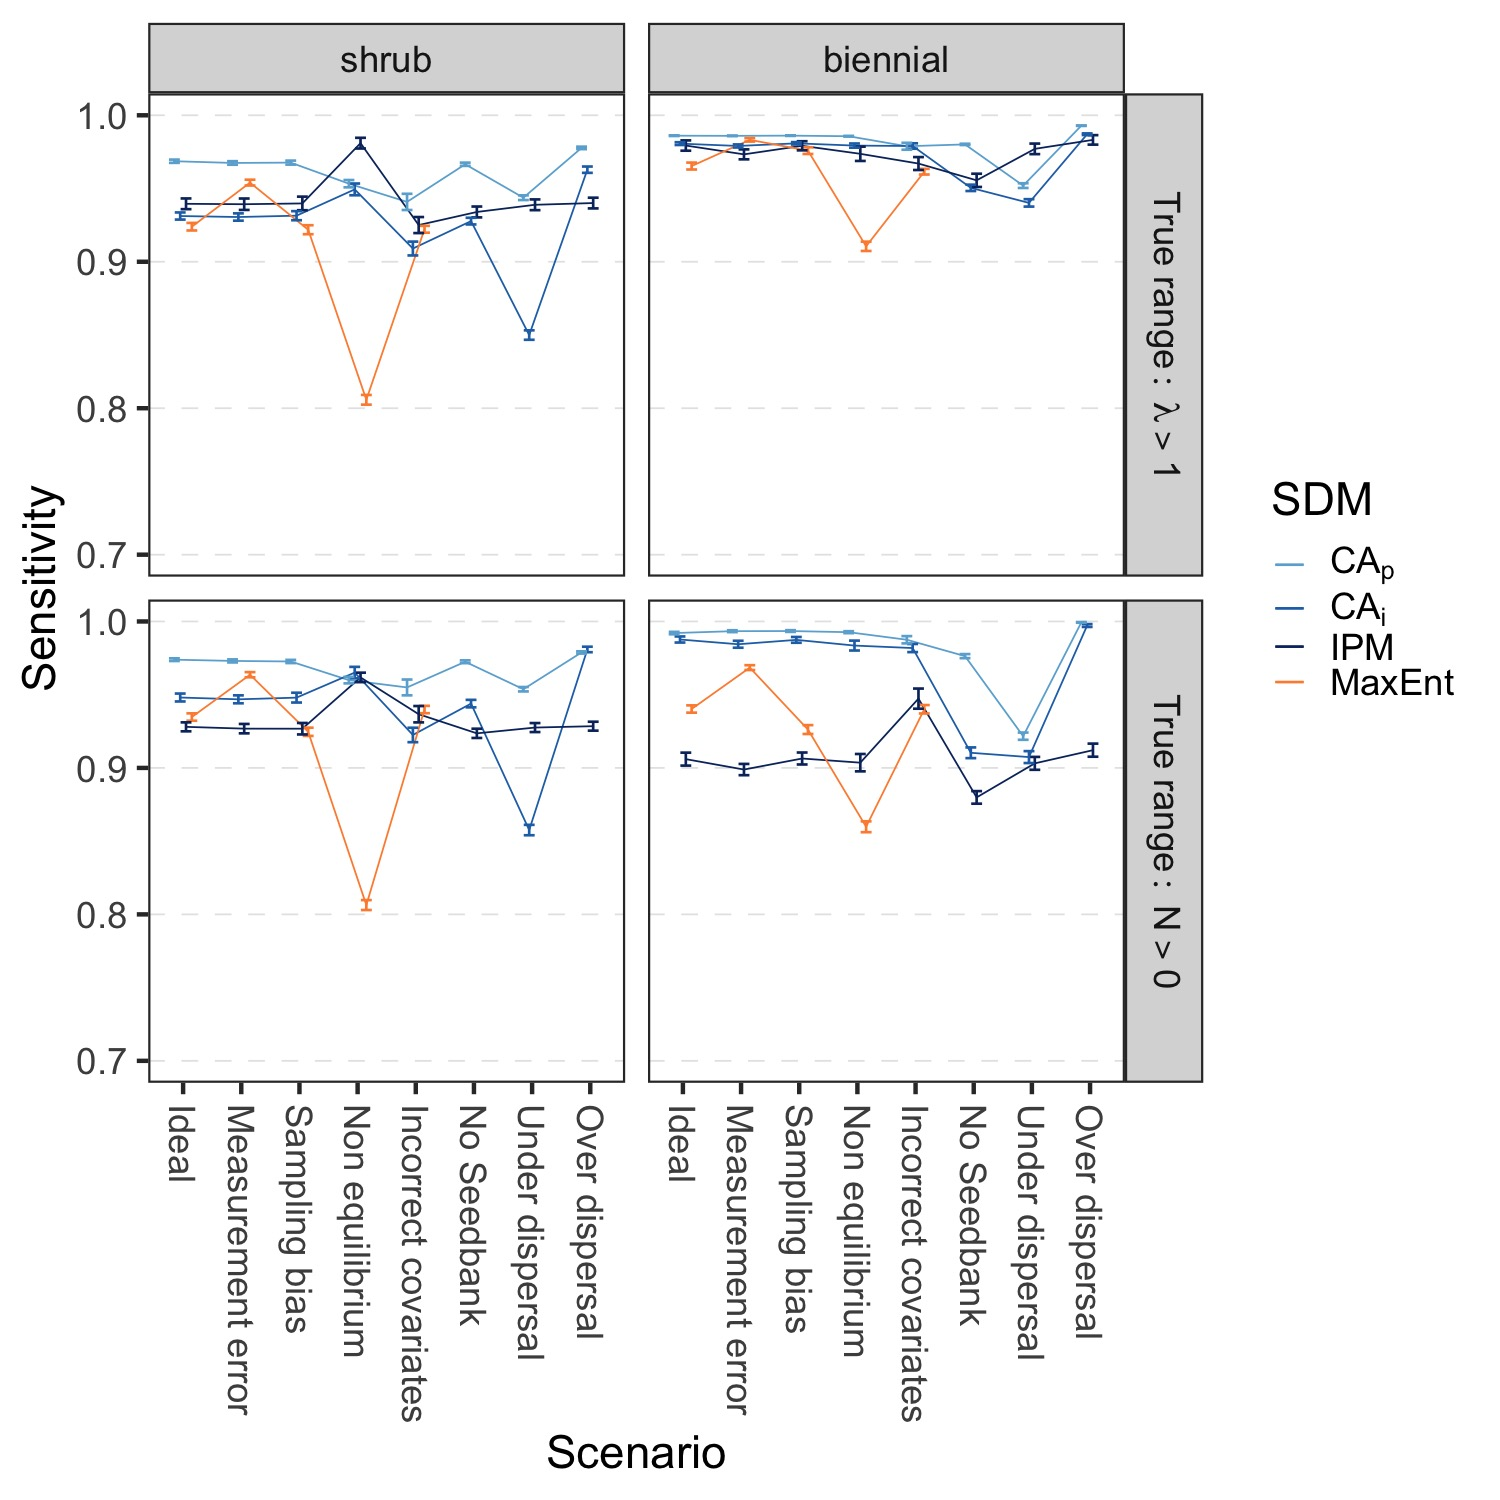
\includegraphics[width=.75\linewidth]{../../figs/Supp_Sens_mn+CI.jpg}
    \caption{\label{fig:SensitivityMed} Sensitivity mean and 95\% confidence intervals across 100 sampled data sets for each SDM and scenario, compared to true distributions defined by $\lambda > 1$ and $N > 0$. Scenarios include: no sampling or modeling issues (ideal), sampling issues (measurement error, sampling bias, non-equilibrium), and modeling issues (incorrect covariates, no seed bank, under dispersal, over dispersal). Sensitivity represents the proportion of true presences that were correctly predicted as presences.}
\end{figure}

\begin{figure}
    \centering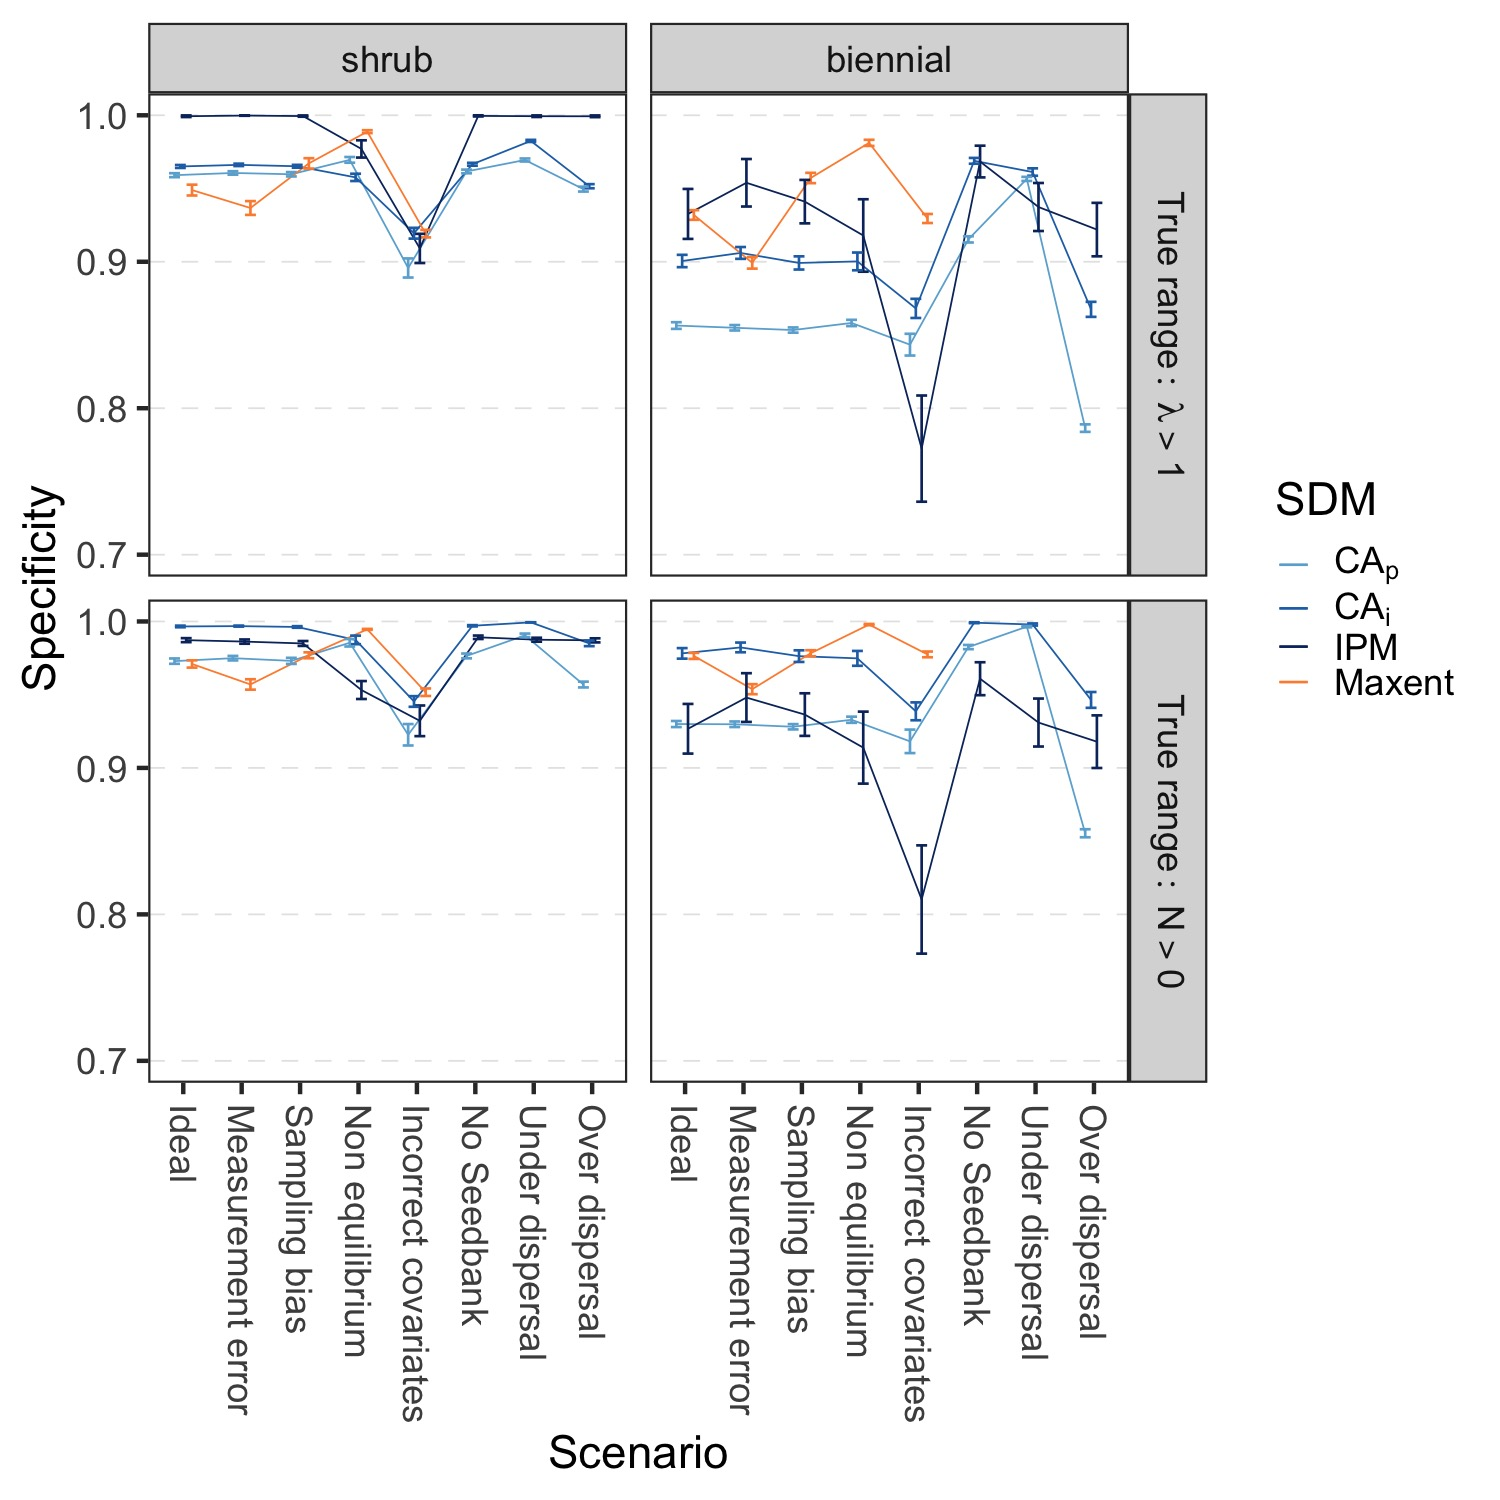
\includegraphics[width=.75\linewidth]{../../figs/Supp_Spec_mn+CI.jpg}
    \caption{\label{fig:SpecificityMed} Specificity mean and 95\% confidence intervals across 100 sampled data sets for each SDM and scenario, compared to true distributions defined by $\lambda > 1$ and $N > 0$. Scenarios include: no sampling or modeling issues (ideal), sampling issues (measurement error, sampling bias, non-equilibrium), and modeling issues (incorrect covariates, no seed bank, under dispersal, over dispersal). Specificity represents the proportion of true absences that were correctly predicted as absences.}
\end{figure}

\newpage
\subsection{Scenario effects}

Some scenarios, such as \emph{non-equilibrium} for MaxEnt or
\emph{under-dispersal} for the process-based models, result in
consistent under-prediction, as seen by a decline in sensitivity and an
increase in specificity. In contrast, \emph{incorrect covariates} has
more complex effects, leading to a decline in both sensitivity and
specificity in the process-based models. In this case, not only are
presences more poorly predicted, but absences are more poorly predicted
as well.

\begin{figure}
    \centering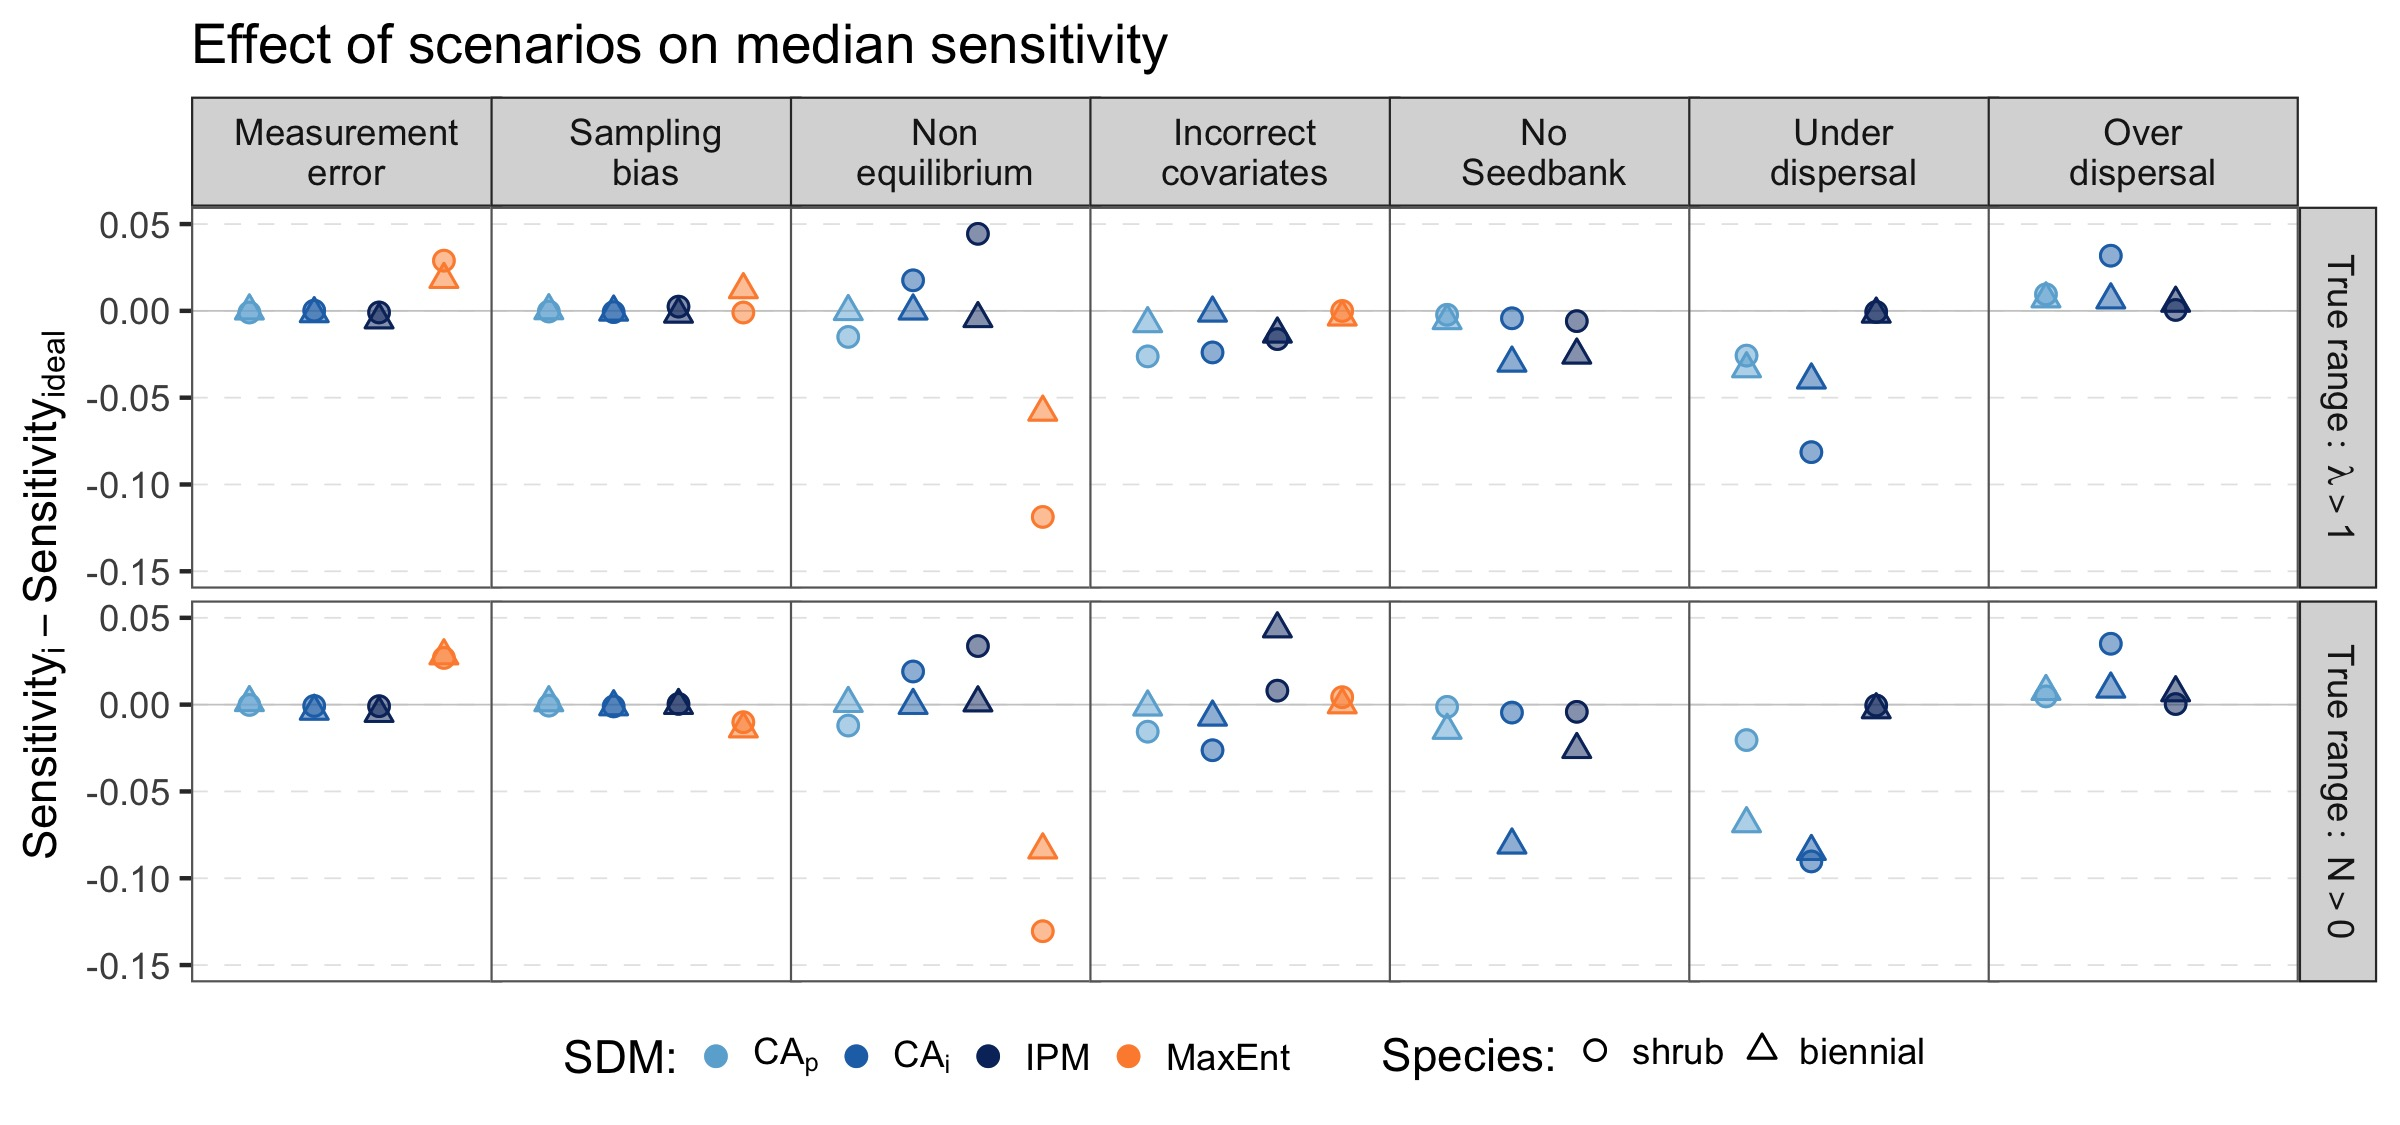
\includegraphics[width=.9\linewidth]{../../figs/Supp_SensvIdeal.jpg}
    \caption{\label{fig:SensitivityvIdeal} Effect of scenario on median sensitivity relative to the \emph{ideal} scenario. Sensitivity represents the proportion of true presences that were correctly predicted as presences.}
\end{figure}

\begin{figure}
    \centering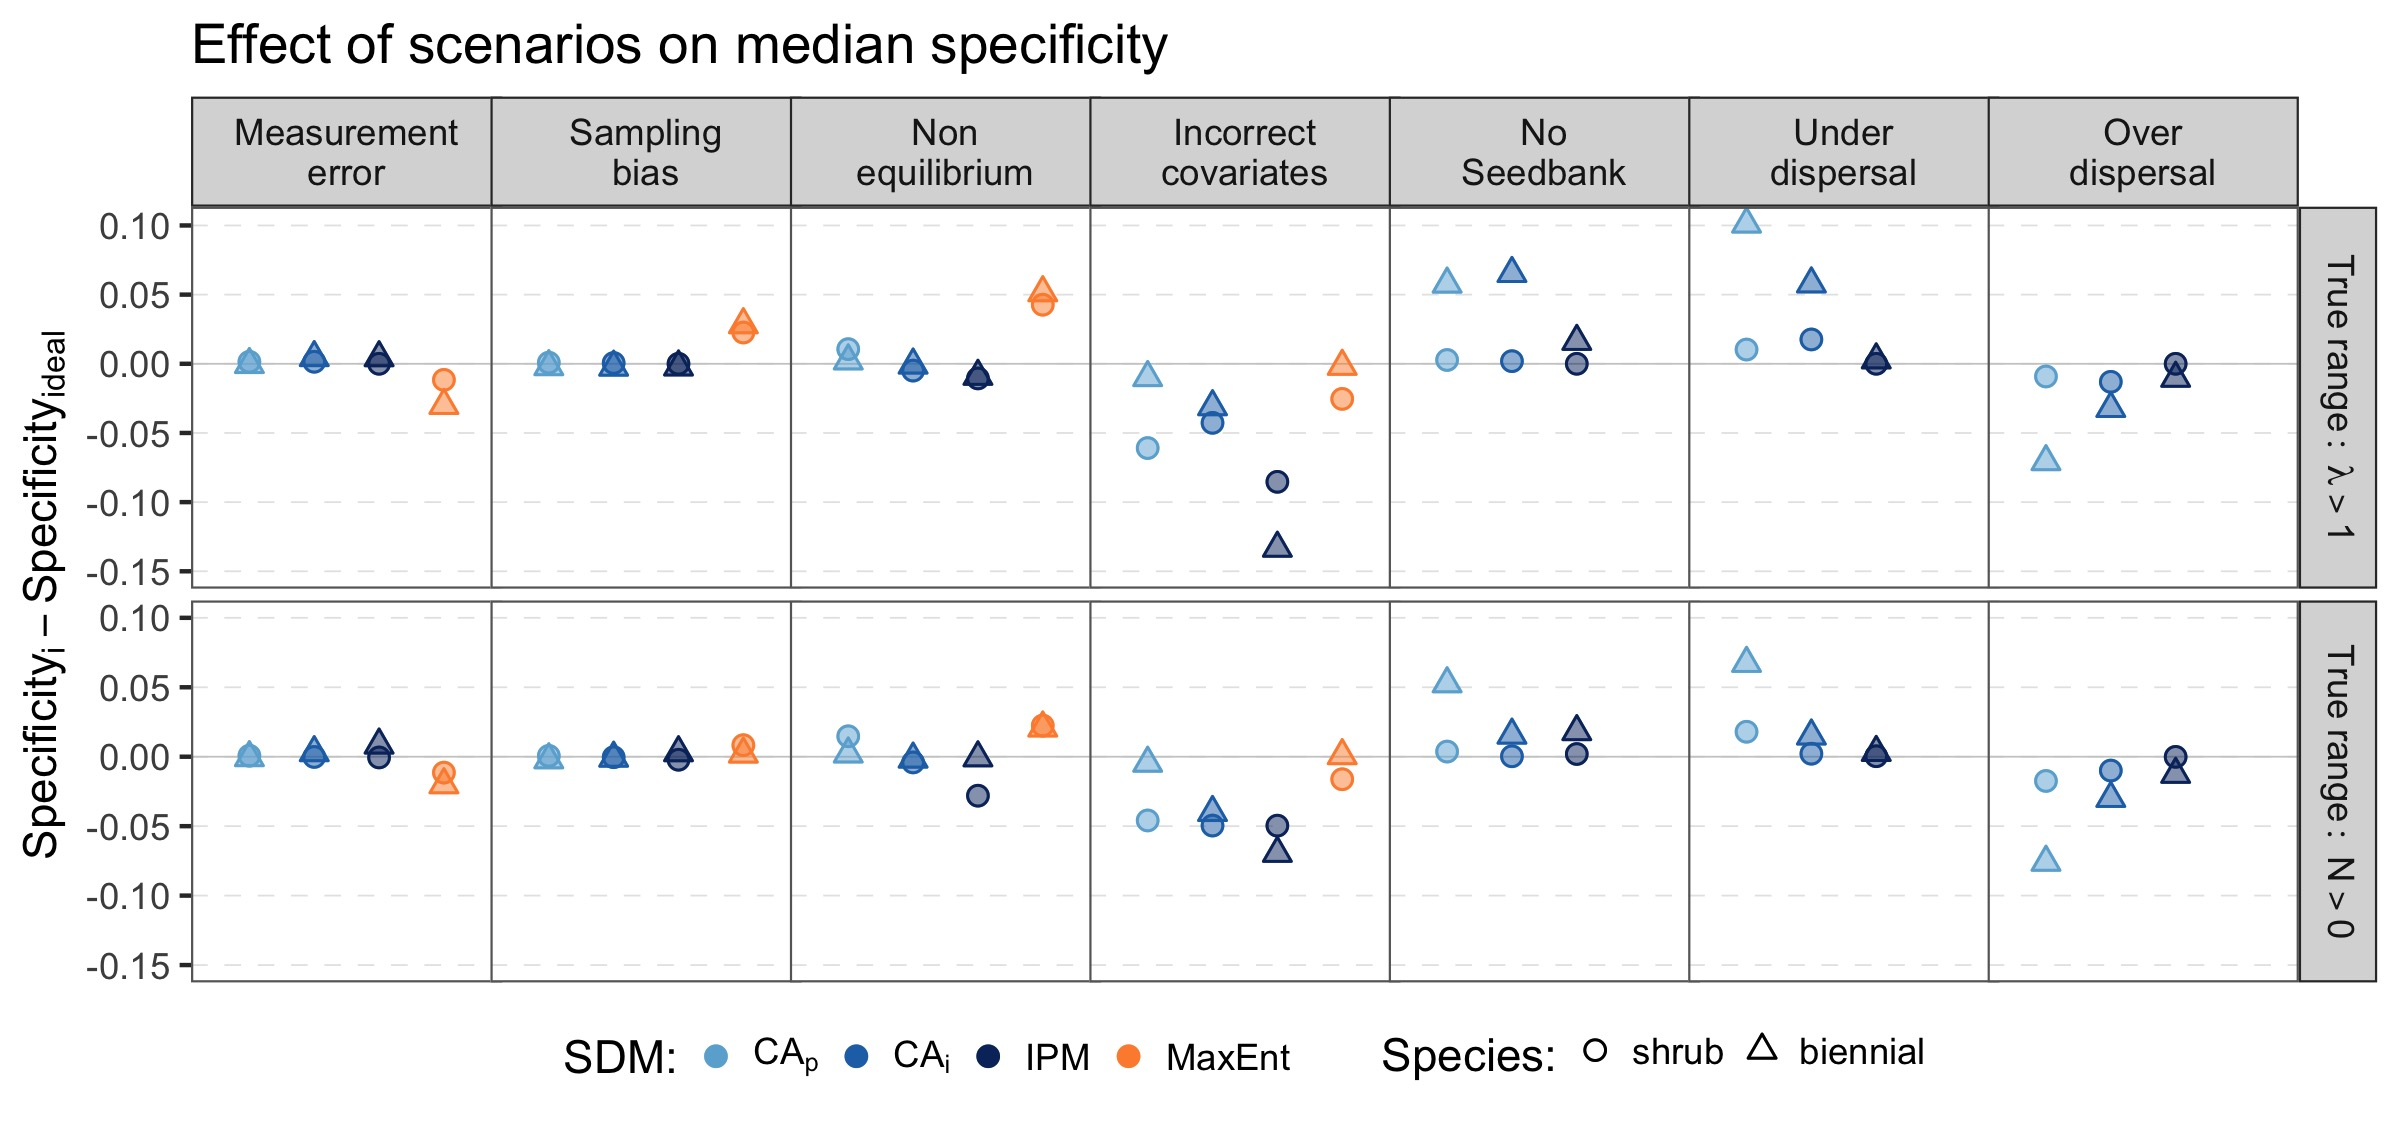
\includegraphics[width=.9\linewidth]{../../figs/Supp_SpecvIdeal.jpg}
    \caption{\label{fig:SpecificityvIdeal} Effect of scenario on median specificity relative to the \emph{ideal} scenario. Specificity represents the proportion of true absences that were correctly predicted as absences.}
\end{figure}

\begin{center}\rule{0.5\linewidth}{\linethickness}\end{center}

\newpage
\section{Estimated slopes}

The IPM and CA\textsubscript{i} models fit regressions of the same form
as the generative models, and so error in the estimated slopes can be
directly compared. The pattern of accuracy across scenarios reflects the
observed trends in TSS. The effect of data scenario is minimal, with the
exception of non-equilibrium for the shrub. The slopes clearly show the
improvement from sampling newer populations with a broader age
distribution, relative to all other scenarios where populations tended
to be older. This effect is absent from the biennial regressions, as
individuals are not long-lived.

\begin{figure}
    \centering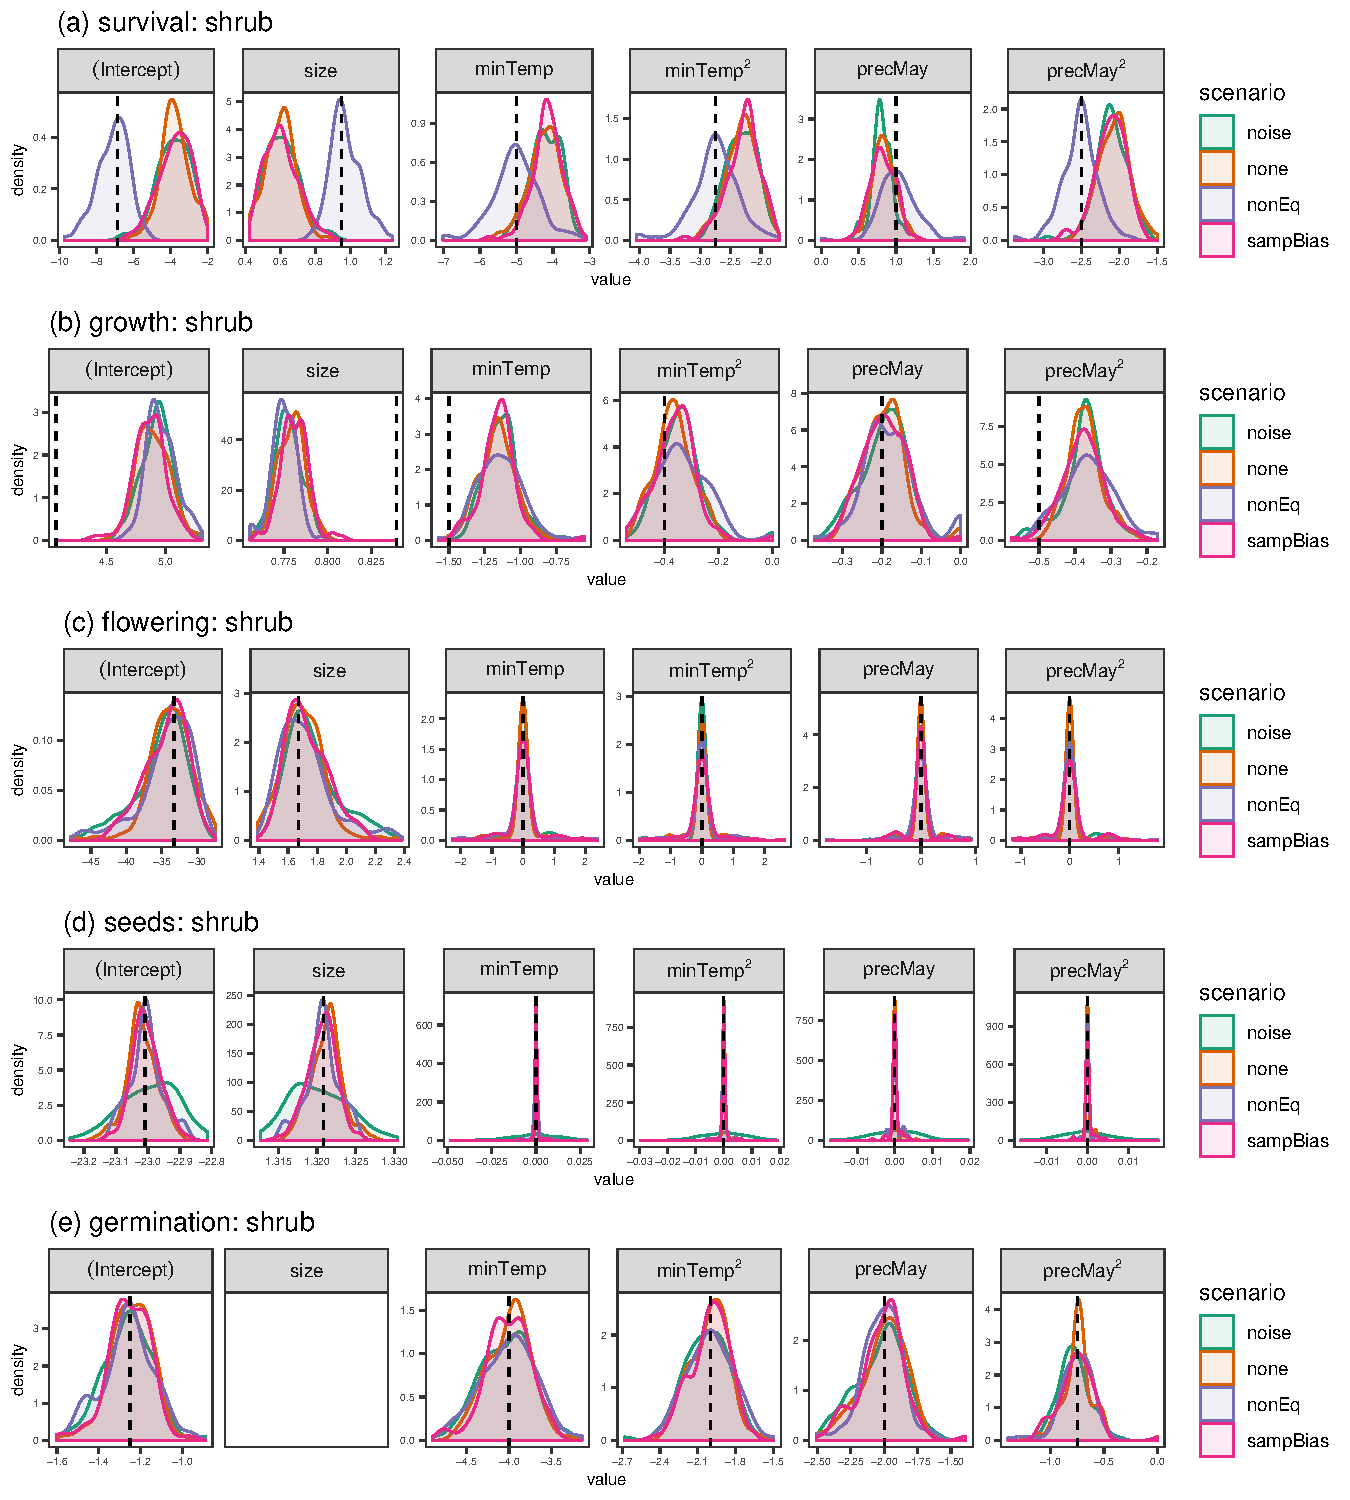
\includegraphics[width=\linewidth]{../../figs/diag/slope_dens_shrub.pdf}
    \caption{\label{fig:slopesShrub} Effect of data scenario on slope estimates for the shrub. Survival regressions for the shrub are parameterized more accurately when using \emph{non-equilibrium} populations which contain a more even size distribution. Note that the axes vary among panels.}
\end{figure}

\begin{figure}
    \centering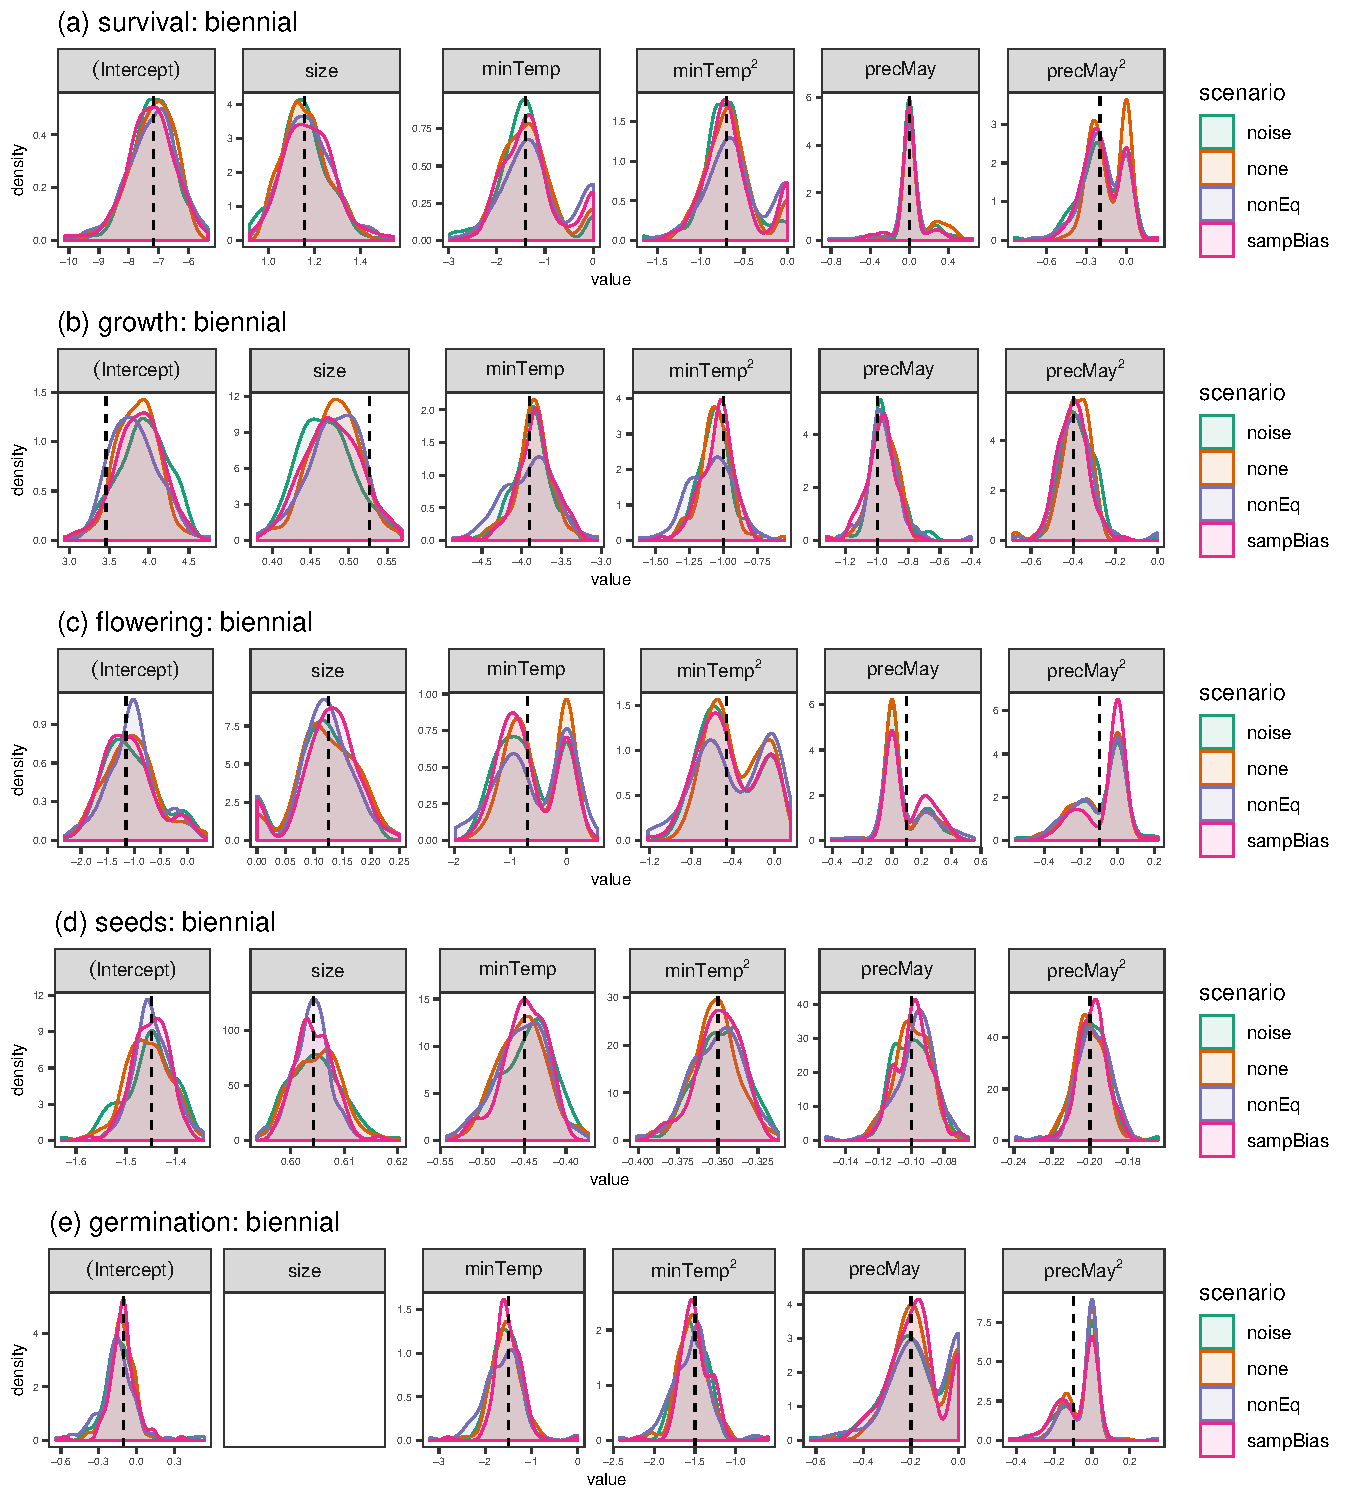
\includegraphics[width=\linewidth]{../../figs/diag/slope_dens_biennial.pdf}
    \caption{\label{fig:slopesBiennial} Effect of data scenario on slope estimates for the biennial Regressions are parameterized consistently with minimal differences among data scenarios. Peaks at 0 represent data sets where the optimal model did not include that term. Note that the axes vary among panels.}
\end{figure}


\end{document}
